% This is samplepaper.tex, a sample chapter demonstrating the
% LLNCS macro package for Springer Computer Science proceedings;
% Version 2.21 of 2022/01/12
%
\documentclass[runningheads]{llncs}
%
\usepackage[T1]{fontenc}
% T1 fonts will be used to generate the final print and online PDFs,
% so please use T1 fonts in your manuscript whenever possible.
% Other font encondings may result in incorrect characters.
%
% \usepackage{times} Do not use this
\usepackage{latexsym}
\usepackage{amssymb}
\usepackage{graphicx}
\usepackage{booktabs}

% Pseudocode
\usepackage{amsmath}
\usepackage{algorithm}
\usepackage{algpseudocode}

\usepackage{graphicx}
% Sort and compress numeric citations in Springer proceedings style.
\usepackage{cite}
\usepackage[hidelinks]{hyperref}
\usepackage{bbding}
% Used for displaying a sample figure. If possible, figure files should
% be included in EPS format.
%
% Keep citations, hyperlinks, and bibliography URLs black.

\usepackage{color}
\renewcommand\UrlFont{\color{blue}\rmfamily}
% \urlstyle{same}
%
\begin{document}
% \pagestyle{empty}
\pagenumbering{gobble}
%
\title{LLM-Assisted Intent-Aware Multimodal Video Retrieval with Diagnostic-Event Temporal Search}
%
\titlerunning{Intent-Aware Video Retrieval with Temporal Search}
% If the paper title is too long for the running head, you can set
% an abbreviated paper title here
%
% \author{First Author\inst{1}\orcidID{0000-1111-2222-3333} \and
% Second Author\inst{2,3}\orcidID{1111-2222-3333-4444} \and
% Third Author\inst{3}\orcidID{2222--3333-4444-5555}}
%
\newcommand{\corrmark}{\unskip$^{\star}$}
\newcommand{\equalcontrib}{\textsuperscript{\dagger}}

\author{
Duc Minh Le\inst{1,2}\fnmsep
\thanks{Corresponding authors}
% \thanks{These authors contributed equally to this work.}
\and
An Thien Tran Nguyen\inst{1,2}
\and
Khuong Xuan Dinh\inst{1,2}\fnmsep\corrmark
\and
Loc Thanh Duong\inst{1,2}
\and
Phuong Hong Tran\inst{1,2}
\and
Thang Minh To\inst{1,2}
}
\authorrunning{D. M. Le et al.}



\institute{
Faculty of Information Technology, University of Science,
Ho Chi Minh City, Vietnam\\
\and
Vietnam National University Ho Chi Minh City, Vietnam
\email{
\{lmduc23,nttan23,dxkhuong23,dtloc23,thphuong23,tmthang23\}
@clc.fitus.edu.vn
}\\
\textit{The order of authors does not reflect the level of contribution.}
}


%



\maketitle              % typeset the header of the contribution
%
\begin{abstract}
Interactive video retrieval is challenged by query-dependent multimodal evidence, ambiguous object descriptions, incomplete frame coverage, and temporal retrieval biased toward isolated high-scoring frames. We present a multimodal retrieval system for the AI Challenge 2026 that addresses these issues without requiring large-scale task-specific training. Our main contributions are: (1) an LLM-based retrieval planner that adaptively routes each query between semantic retrieval and textual evidence from captions, ASR, and OCR; (2) evidence-oriented reasoning that decomposes ambiguous descriptions into retrievable entities, actions, attributes, and lexical cues; and (3) Diagnostic-Event-Video-First (DEV), a coarse-to-fine global-to-local strategy that improves video coverage through adaptive sampling and performs annotation-aware temporal refinement to recover ordered event sequences rather than isolated frames. Experiments show that DEV outperforms the compared temporal retrieval methods from Recall@10 onward. In the official AIC 2026 preliminary evaluation, our system achieved $88.63\%$ of the maximum available score and qualified as a finalist for the AIC 2026 final round.
\keywords{Event retrieval  \and Temporal Search \and LLM-Assisted Intent-Aware Retrieval \and Query-Adaptive Retrieval}
\end{abstract}

\section{Introduction}
\label{sec:introduction}

Interactive video retrieval requires locating relevant moments from large
video collections using heterogeneous evidence, including visual content,
speech, scene text, and temporal context. This problem is particularly
challenging in benchmarks such as the Video Browser Showdown, Lifelog Search
Challenge, and Ho Chi Minh City AI Challenge 2026
(AIC 2026)\footnote{\url{https://aichallenge.hochiminhcity.gov.vn/}}, where
queries may involve complex scenes, named entities, ambiguous objects, or
temporally ordered events
\cite{schoeffmann2014video,tran2025state,do2027abstraction}.
Recent systems combine vision--language embeddings with OCR, ASR, captions,
and temporal retrieval
\cite{nguyen2027aithena,nguyen2027vortex}; however, fixed retrieval
strategies remain limited when the relevance of these evidence sources varies
across queries.

First, semantic and lexical evidence are query dependent: visual
descriptions favor vision--language retrieval, whereas names, dialogue,
numbers, and scene text are better captured by captions, ASR, or OCR.
Fixed fusion weights may therefore introduce unnecessary noise, particularly
without large-scale task-specific training data. Second, challenge queries
often describe objects indirectly through attributes, actions, or context
rather than explicit names, making their observable evidence difficult to
capture through direct query embedding. Third, sparse keyframe extraction may
omit short but critical events. In temporal retrieval, direct top-$K$ frame
search can further concentrate results around a few high-scoring frames,
reducing the coverage of videos containing the complete event sequence.

To address these issues, we develop a multimodal video retrieval system for
AIC 2026 that combines \emph{LLM-assisted retrieval planning} with
coarse-to-fine temporal search. The planner interprets each query, transforms
ambiguous descriptions into retrievable visual and textual evidence,
generates complementary semantic and lexical views, and assigns
query-dependent weights to visual, caption, ASR, and OCR retrieval. For
temporal queries, it further decomposes the description into ordered events
and estimates their importance and diagnostic value. We then introduce
\emph{Diagnostic-Event-Video-First} (DEV) retrieval, which uses global event
evidence to identify promising videos before performing video-local temporal
refinement under chronological and temporal-gap constraints.

Our main contributions are threefold. First, we introduce a
\emph{query-adaptive multimodal retrieval} framework with an LLM-based
planner that routes queries between semantic and textual retrieval and
adaptively weights visual, caption, ASR, and OCR evidence without
task-specific model training. Second, we propose
\emph{evidence-oriented query reasoning}, in which the planner decomposes
ambiguous or indirectly described concepts into observable entities,
actions, attributes, and lexical cues, thereby generating complementary
views for vector and metadata retrieval. Third, we introduce
\emph{Diagnostic-Event-Video-First (DEV)}, a coarse-to-fine global-to-local
retrieval strategy that uses diagnostic events to improve candidate-video
coverage before event-level temporal refinement, reducing the bias of
direct top-$K$ frame retrieval toward isolated high-scoring frames.

Experimental results show that DEV outperforms the compared temporal
retrieval strategies from Recall@10 onward, indicating improved preservation
of relevant videos at practical retrieval depths. In the official AIC 2026
preliminary evaluation, our complete system achieved $88.63\%$ of the maximum
available score and qualified as a finalist for the AIC 2026 final round.
\section{Related Work}
\label{sec:related-work}

Recent interactive video retrieval systems increasingly combine visual embeddings, textual metadata, and temporal context to support complex search scenarios. AIthena-Vision integrates Perception Encoder features with OCR, ASR, object detection, LLM-based query expansion, and Adaptive Temporal Search for multi-event retrieval \cite{nguyen2027aithena}. Its strength lies in diversifying query perspectives while exploiting multiple evidence sources. Vortex similarly combines CLIP and SigLIP2 through reciprocal rank fusion, together with OCR, captions, speech transcripts, relevance feedback, and temporal reranking \cite{nguyen2027vortex}. VideoEase also adopts multimodel fusion using CLIP, BLIP2, and OpenCLIP, and supports temporal search between two scenes \cite{tran2025videoease}. These systems show the effectiveness of multimodal evidence fusion, but modality importance is generally not explicitly determined from the semantic structure of each query, and multi-event temporal alignment remains only partially addressed.

Other approaches focus on richer event-level and contextual representations. U-CESE retrieves coherent clips using lightweight keyframe extraction, context-aware caption propagation, and a unified clipping strategy \cite{le2026ucese}. MEMORIA combines dense annotations, CLIP retrieval, event segmentation, and LLM-assisted query analysis to improve lifelog search \cite{gago2025memoria}, while LifeSearch incorporates multimodal metadata and structured spatial-temporal information \cite{piramanayagam2025lifesearch}. SnapSeek 3.0 further introduces scene-graph-based retrieval and temporal consistency mechanisms \cite{hole2025snapseek}. T-EAGLE represents sequences of frames as textual action narratives, enabling retrieval at the event rather than isolated-frame level \cite{nguyenho2025teagle}. U-Cker complements these methods through interfaces that support interactive exploration of temporally related lifelog moments \cite{ueki2026ucker}. Although these approaches improve contextual and temporal retrieval, they mainly depend on predefined temporal modes, pre-generated event representations, or temporal grouping after retrieval.

Our system builds on these advances by connecting query understanding directly to evidence selection and temporal sequence construction. An LLM generates semantic rewrites, lexical queries, event decompositions, and modality-specific evidence weights before retrieval. Diagnostic-Event-Video-First search then uses event importance and preliminary retrieval evidence to identify promising videos, after which bounded beam search explicitly aligns candidates under chronological and temporal-gap constraints. The main distinction is therefore not any individual component, but the integration of query-dependent multimodal weighting, diagnostic-event-guided retrieval, and explicit multi-event temporal alignment within a unified pipeline.
\section{Architecture}

\label{sec:architecture}

% FAST-COMPILE: system-overview image disabled; restore this block for camera-ready.
\iffalse
\begin{figure*}[h]
    \centering
    % Save the supplied image as figures/system_overview.png
    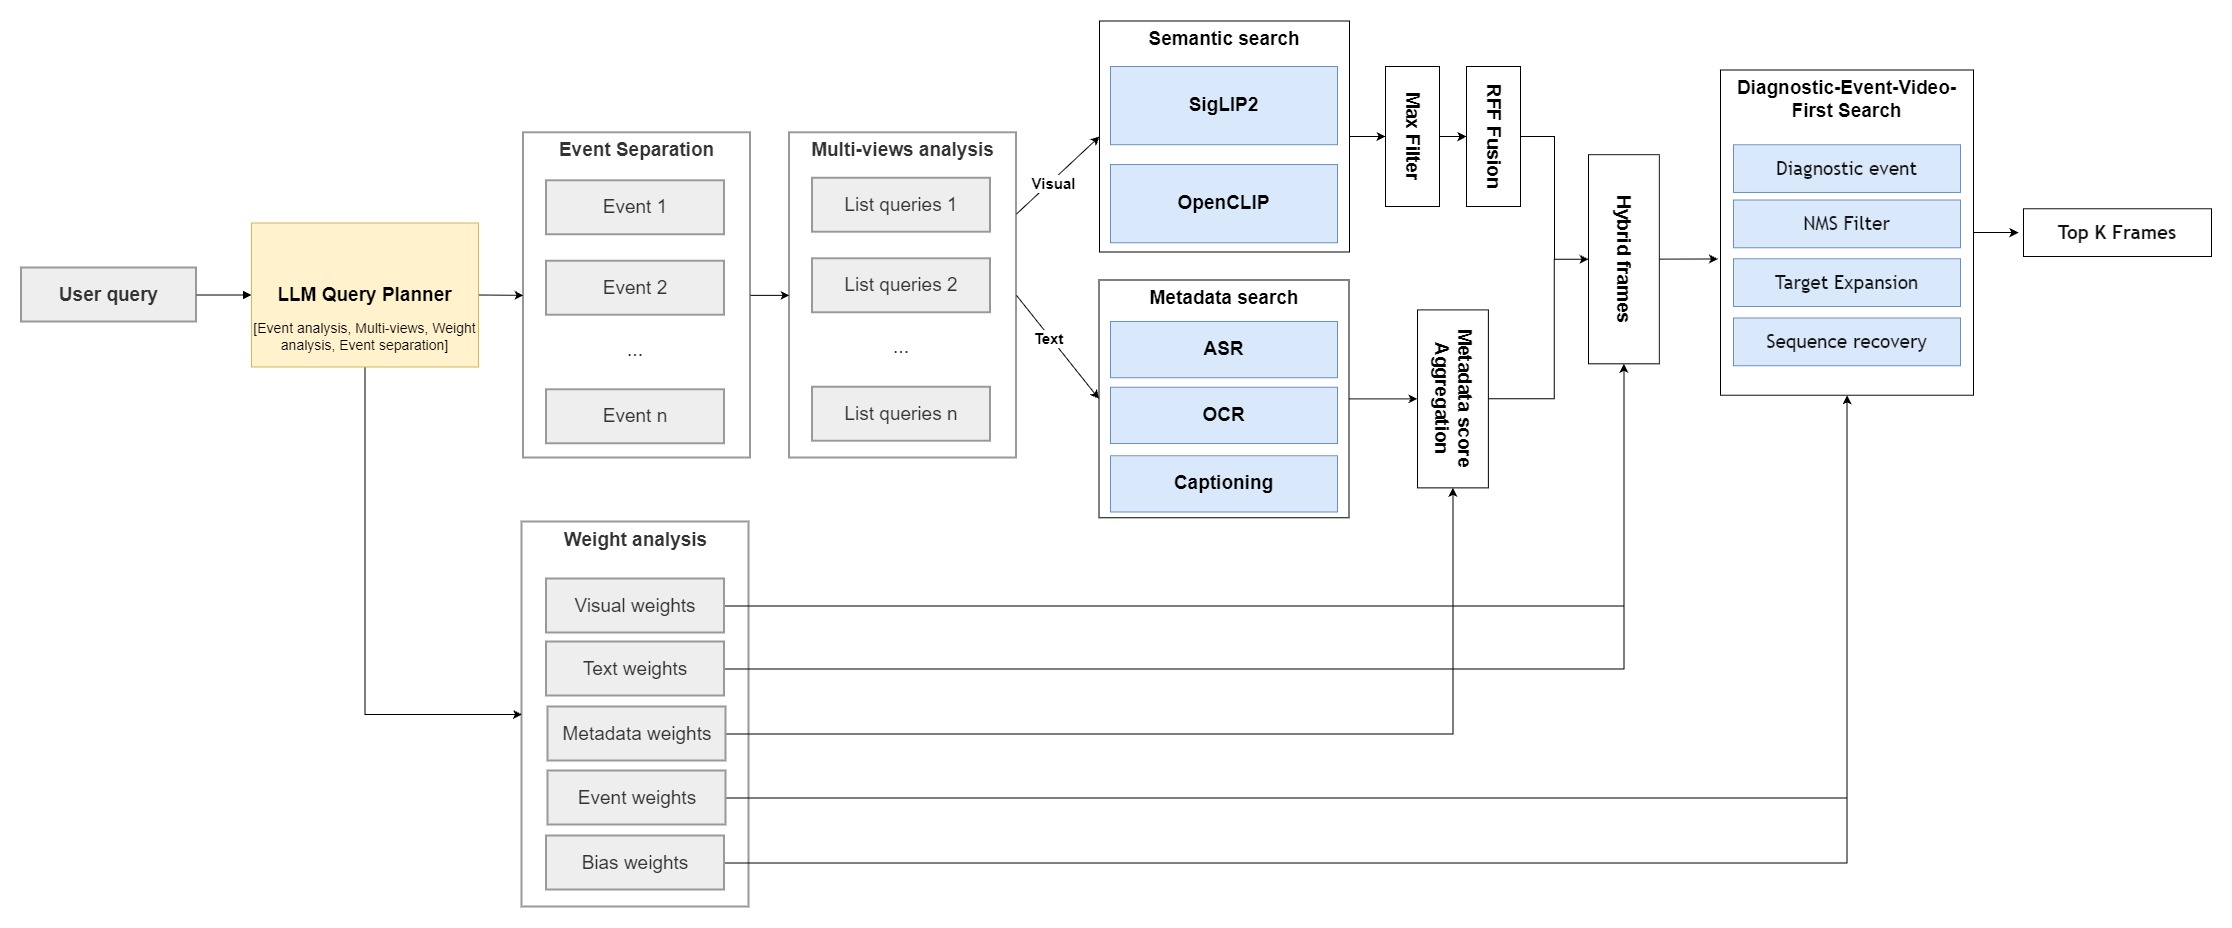
\includegraphics[width=\textwidth]{figures/search_pipeline_v1.jpg}
    \caption{Overview of the proposed multimodal video search pipeline.}
    \label{fig:system-overview}
\end{figure*}
\fi

Figure~\ref{fig:system-overview} illustrates the proposed multimodal
retrieval pipeline. Given a query, the LLM planner generates semantic and
lexical views, assigns modality-specific weights, and, for temporal queries,
decomposes the description into ordered events with importance and diagnostic
scores. Visual and metadata evidence are retrieved in parallel and fused into
hybrid frame candidates, with multiple visual branches combined by max-view
aggregation and reciprocal rank fusion. For temporal queries, DEV first uses
diagnostic-event evidence to select promising videos, then performs
video-local retrieval with temporal redundancy reduction, chronological and
gap constraints, and sequence scoring to produce the final top-$K$ results.


\subsection{Data Processing}
\label{sec:data_processing}

% FAST-COMPILE: data-processing image disabled; restore this block for camera-ready.
\iffalse
\begin{figure}[H]
\centering
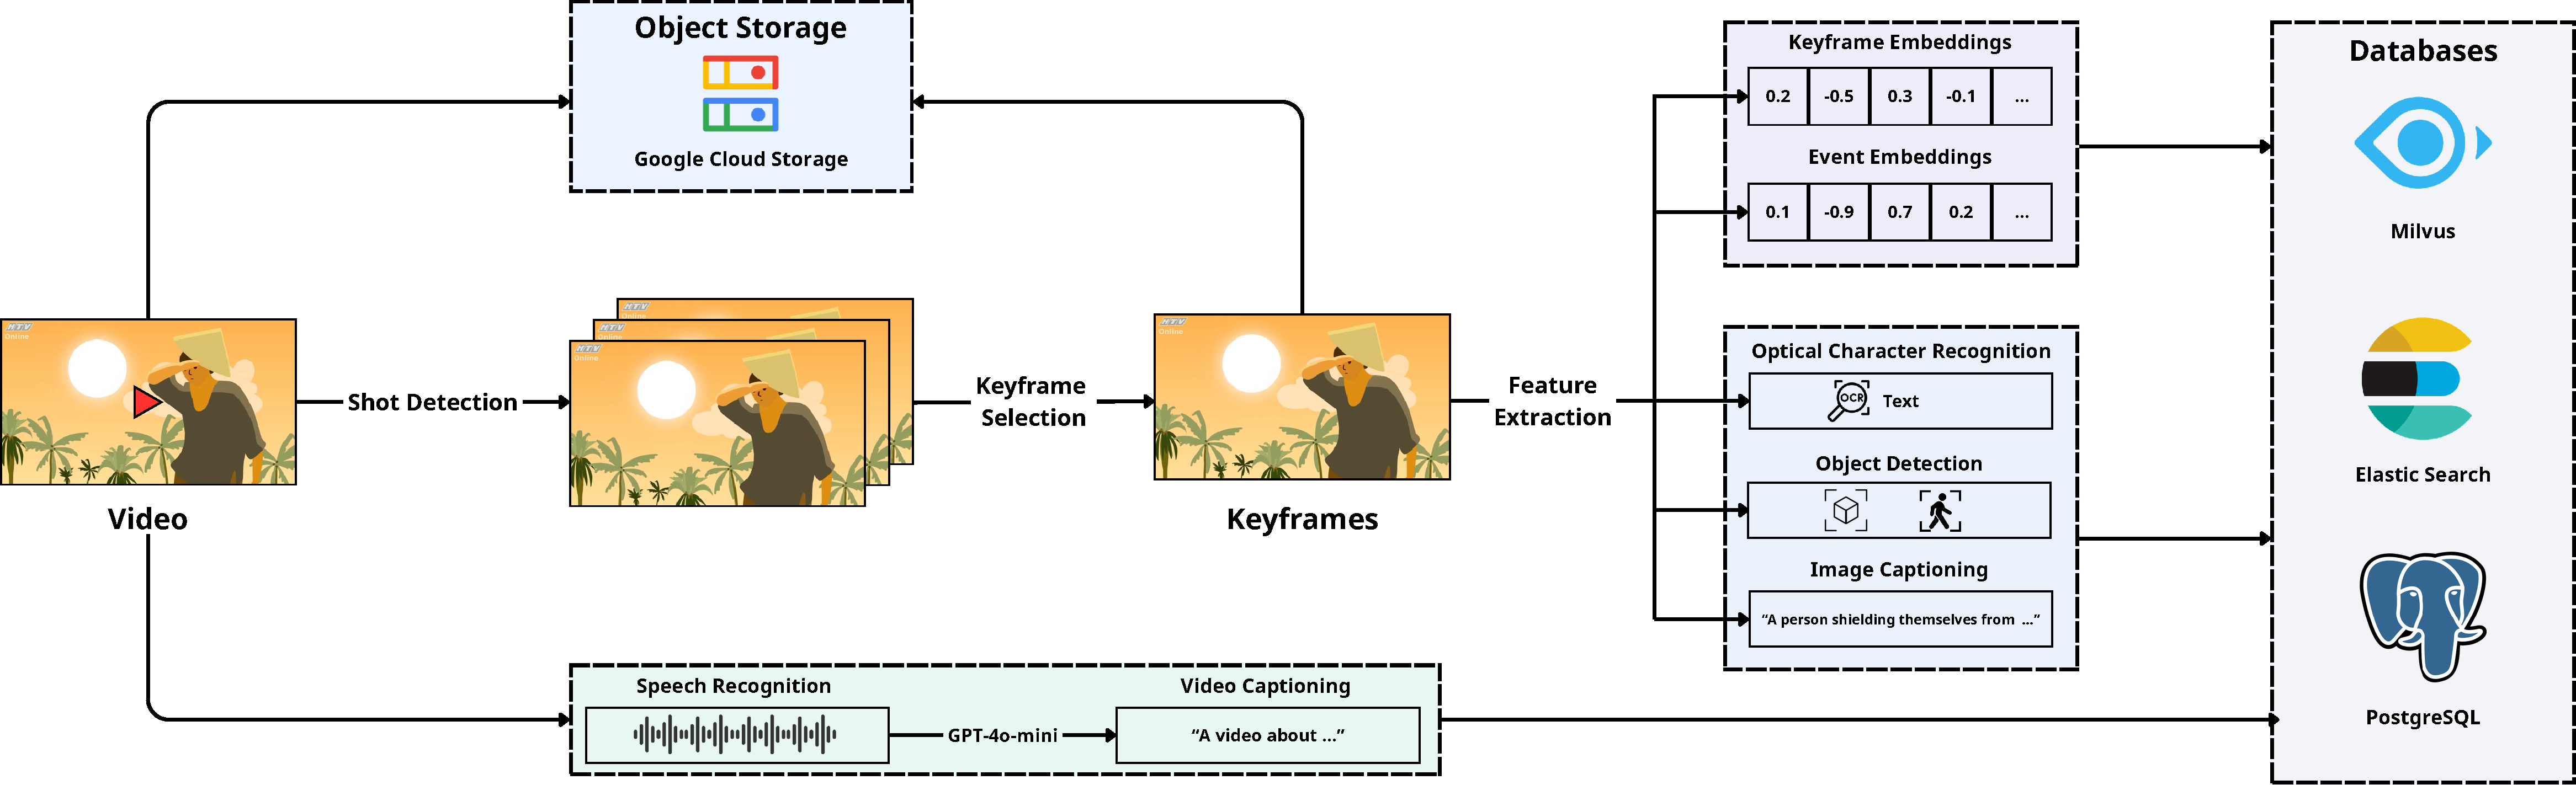
\includegraphics[width=\linewidth]{figures/data_processing_pipeline_new.pdf}
\caption{Overview of the proposed data preprocessing pipeline.}
\label{fig:data-processing-pipeline}
\end{figure}
\fi

Figure~\ref{fig:data-processing-pipeline} illustrates our data processing pipeline. Given the raw videos, we first employ AutoShot~\cite{zhu2023autoshot} to identify shot boundaries. For each detected shot, three representative frames are sampled from the beginning, middle, and end portions. Compared with using a single representative frame, this strategy provides broader temporal coverage and reduces the risk of missing transient but retrieval-relevant visual information. The extracted keyframes, together with the original videos, are stored in Google Cloud Storage~\cite{googlecloudstorage2026} for efficient media access and visualization in the retrieval interface.

\paragraph{Visual representation.}
Each keyframe is independently encoded using OpenCLIP ViT-H/14-quickgelu with DFN-5B weights~\cite{ilharco2021openclip,fang2024dfn} and SigLIP 2 SO400M/16~\cite{tschannen2025siglip2}. The DFN-5B checkpoint provides a strong CLIP-based image--text representation learned from carefully filtered large-scale image--text data, whereas SigLIP 2 improves semantic image--text retrieval and provides stronger multilingual and localized visual representations. Using these complementary embedding spaces increases the robustness of subsequent semantic retrieval. To obtain event-level representations, temporally adjacent keyframes whose embedding similarity exceeds a threshold $T$ are grouped into the same event. Given an event containing $N$ keyframes with embeddings $\{\mathbf{v}_i\}_{i=1}^{N}$, its representation is computed as
\begin{equation}
    \mathbf{v}_{e}=\frac{1}{N}\sum_{i=1}^{N}\mathbf{v}_{i}.
\end{equation}
This temporal aggregation reduces redundant frame-level representations while preserving the dominant semantics of each event for event-level retrieval.

\paragraph{Visual semantic enrichment.}
We further enrich each keyframe with complementary textual and object-level information. For optical character recognition (OCR), PaddleOCR~\cite{du2020ppocr} is employed for text detection, followed by VietOCR~\cite{vietocr} for Vietnamese text recognition. The recognized text is subsequently normalized using the vietnamese-correction-v2 model~\cite{vietnameseCorrectionV2} to mitigate spelling and recognition errors. Object information is extracted using the COCO-pretrained YOLO26x detector~\cite{jocher2026yolo26}, which recognizes 80 common object categories. We adopt the largest YOLO26 detection variant to favor detection accuracy during offline preprocessing. In parallel, Qwen3-VL-4B-Instruct~\cite{bai2025qwen3vl} generates keyframe captions describing visible entities, attributes, spatial relations, and interactions, while also providing fine-grained object-level semantic information complementary to YOLO26 detections. This enriches the representation beyond the fixed set of object categories covered by conventional object detection.


\paragraph{Speech and video-level semantics.}
For the audio modality, speech segments are first identified using voice activity detection (VAD) and subsequently transcribed with Whisper Large V3 Turbo~\cite{radford2022whisper,whisperLargeV3Turbo}. VAD suppresses non-speech regions and provides finer speech segmentation, which is particularly useful for retaining short utterances. The resulting transcripts are post-processed by GPT-4o mini~\cite{openai2024gpt4omini} for spelling normalization and English translation. In addition to local frame-level descriptions, we derive a global video-level semantic summary by providing the complete transcript of each video to GPT-4o mini and prompting it to extract its principal content. We refer to this transcript-derived summary as the \emph{video caption}, which complements frame-level visual captions with global conversational context.

\paragraph{Indexing and storage.}
Finally, the resulting multimodal representations are organized according to their retrieval characteristics. Dense keyframe and embeddings are indexed in Milvus~\cite{wang2021milvus} for vector similarity search, while textual metadata, including OCR outputs, captions, object labels, transcripts, and video-level summaries, are indexed in Elasticsearch~\cite{elasticsearch2026} and maintained together with structured metadata in PostgreSQL~\cite{postgresql2026}. This separation enables the retrieval system to efficiently combine visual similarity, textual matching, and structured filtering within a unified multimedia search pipeline.
% \subsection{Data Processing}
% \label{sec:data_processing}

% \begin{figure}[t]
% \centering
% 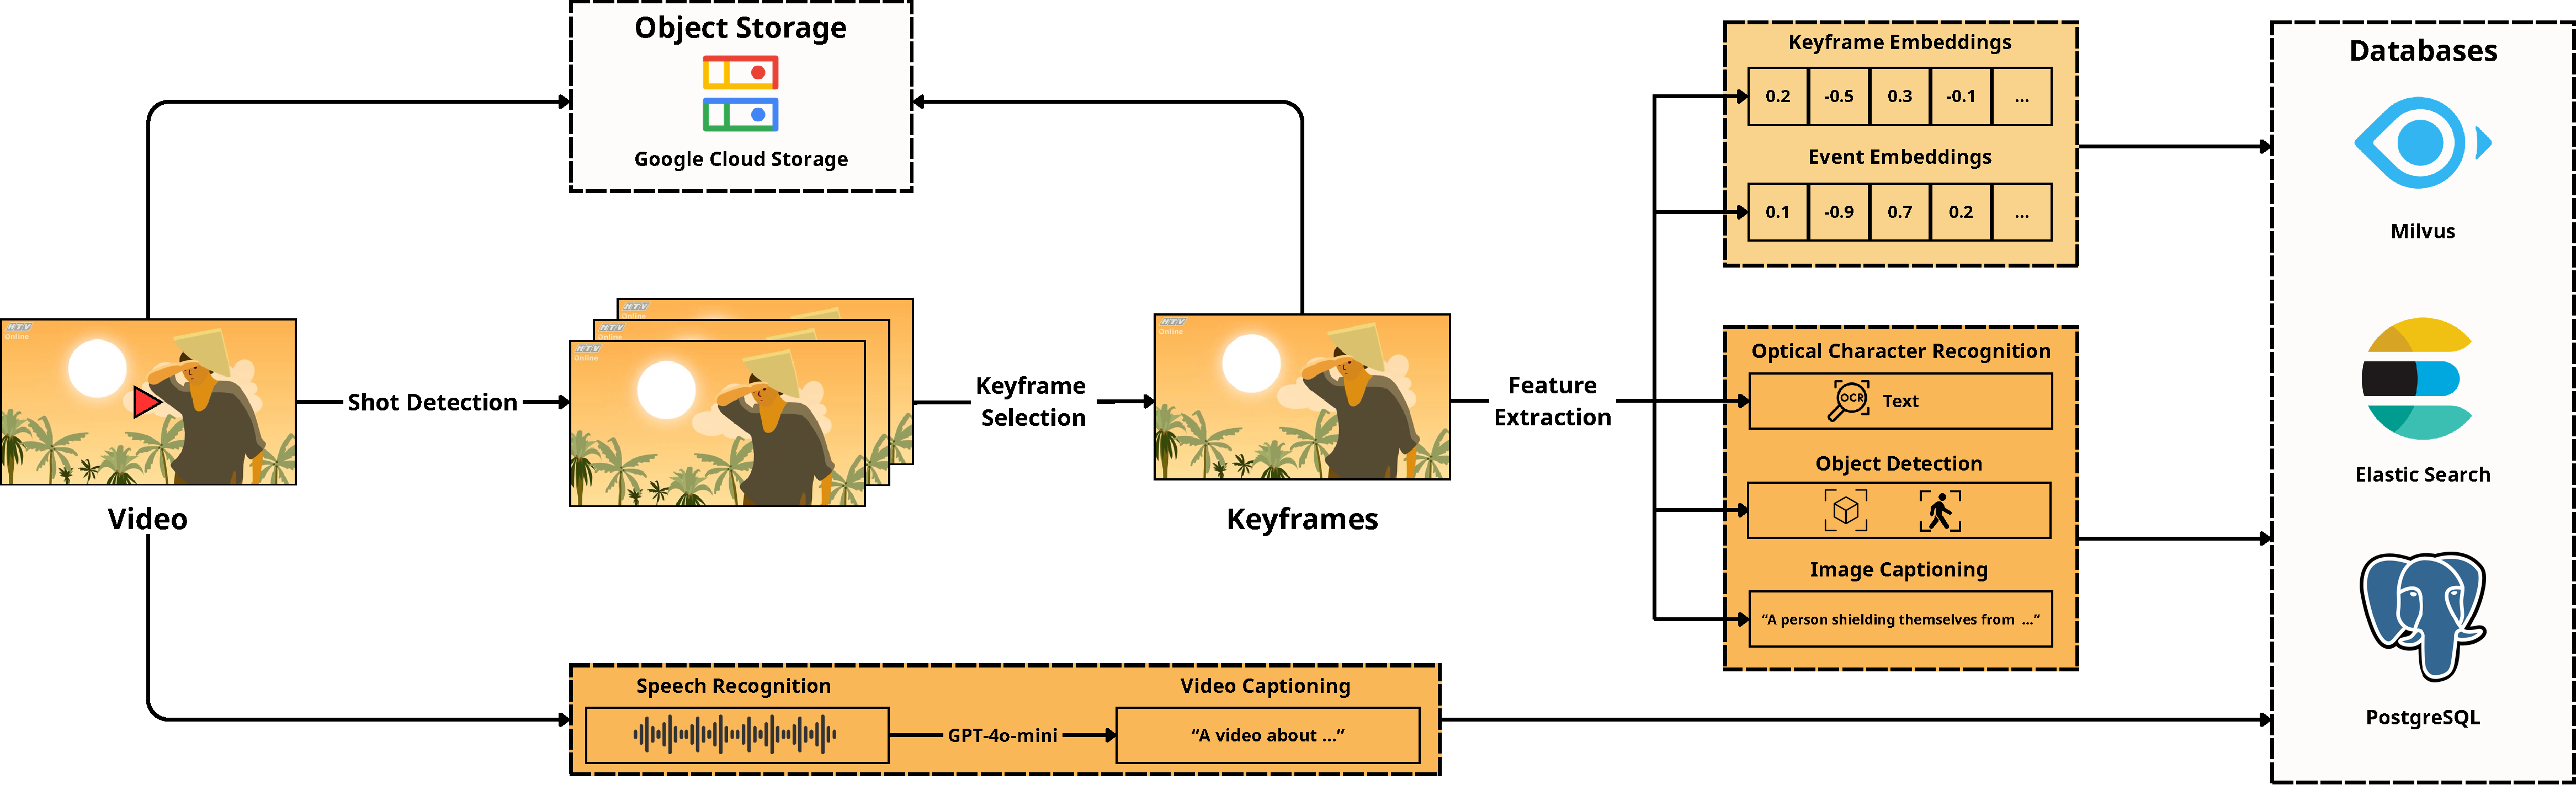
\includegraphics[width=\linewidth]{figures/data_processing_pipeline.pdf}
% \caption{Overview of the proposed data preprocessing pipeline.}
% \label{fig:data-processing-pipeline}
% \end{figure}

% Figure~\ref{fig:data-processing-pipeline} illustrates our data processing pipeline. We use AutoShot~\cite{zhu2023autoshot} to detect shot boundaries and sample three representative frames from the beginning, middle, and end of each shot to improve temporal coverage. We store the original videos and extracted keyframes in Google Cloud Storage~\cite{googlecloudstorage2026}.

% \paragraph{Visual representation.}
% We use OpenCLIP ViT-H/14-quickgelu with DFN-5B weights~\cite{ilharco2021openclip,fang2024dfn} and SigLIP 2 SO400M/16~\cite{tschannen2025siglip2} to encode each keyframe into complementary image--text embedding spaces. We group temporally adjacent keyframes whose embedding similarity exceeds a threshold $T$ into events and use the mean of their embeddings as the event representation.

% \paragraph{Visual semantic enrichment.}
% We use PaddleOCR~\cite{du2020ppocr} for text detection, VietOCR~\cite{vietocr} for Vietnamese text recognition, and vietnamese-correction-v2~\cite{vietnameseCorrectionV2} to normalize OCR errors. We use the COCO-pretrained YOLO26x detector~\cite{jocher2026yolo26} to extract object labels. In parallel, we use Qwen3-VL-4B-Instruct~\cite{bai2025qwen3vl} to generate keyframe captions describing visible entities, attributes, spatial relations, and interactions, providing semantic information beyond the fixed object categories of the detector.

% \paragraph{Speech and video-level semantics.}
% We use voice activity detection (VAD) to identify speech regions and Whisper Large V3 Turbo~\cite{radford2022whisper,whisperLargeV3Turbo} to generate ASR transcripts. We then use GPT-4o mini~\cite{openai2024gpt4omini} to normalize transcription errors and translate the transcripts into English. We also use GPT-4o mini to summarize the complete transcript of each video into a \emph{video caption}, providing global conversational context complementary to frame-level captions.

% \paragraph{Indexing and storage.}
% We use Milvus~\cite{wang2021milvus} to index dense visual embeddings for similarity search and Elasticsearch~\cite{elasticsearch2026} to index OCR text, captions, object labels, ASR transcripts, and video captions. We use PostgreSQL~\cite{postgresql2026} to maintain structured metadata. This organization supports efficient semantic retrieval, textual matching, and structured filtering.

\subsection{Multimodal Retrieval}
\subsubsection{Semantic Vector Retrieval}

We perform semantic retrieval by matching each query against the indexed
keyframe representations described in Section~\ref{sec:data_processing}.
All query and frame embeddings are $\ell_2$-normalized before
cosine-similarity retrieval.

Given the original query and its LLM-generated semantic views
$\{q_j\}_{j=1}^{J}$, each view is independently used to retrieve its
top-$k$ keyframes. For each frame, we retain the strongest evidence
across all query views:
\begin{equation}
s_m(f)=
\max_{\substack{
1\leq j\leq J\\
f\in\mathcal{N}^{(m)}_k(q_j)
}}
\left[
\cos\!\left(
E^{(m)}_{\mathrm{text}}(q_j),
\mathbf{v}^{(m)}_f
\right)
\right]_{+},
\end{equation}
where $\mathcal{N}^{(m)}_k(q_j)$ denotes the top-$k$ results of query
view $q_j$ under embedding space $m$.

When multiple embedding spaces are enabled, we combine their ranked
results using weighted reciprocal rank fusion (RRF)~\cite{cormack2009rrf}:
\begin{equation}
s_{\mathrm{vec}}(f)=
\sum_{m\in\mathcal{M}}
\frac{\beta_m}{K+r_m(f)},
\end{equation}
where $r_m(f)$ is the rank of frame $f$ under embedding space $m$ and
$\beta_m$ controls its contribution.

% We use semantic vector retrieval to align natural-language queries with
% indexed video frames. The visual encoders and offline feature extraction
% procedure are described in Section~\ref{sec:data_processing}. For each
% keyframe $I_f$, its representation under encoder $m$ is $\ell_2$-normalized as
% \begin{equation}
% \mathbf{v}^{(m)}_f =
% \frac{E^{(m)}_{\mathrm{img}}(I_f)}
% {\left\lVert E^{(m)}_{\mathrm{img}}(I_f)\right\rVert_2}.
% \end{equation}
% The resulting representations are stored in separate vector indexes for
% each embedding space.

% At retrieval time, the original query and its LLM-generated semantic
% rewrites $\{q_j\}_{j=1}^{J}$ are encoded using the corresponding text
% encoder:
% \begin{equation}
% \mathbf{z}^{(m)}_j =
% \frac{E^{(m)}_{\mathrm{text}}(q_j)}
% {\left\lVert E^{(m)}_{\mathrm{text}}(q_j)\right\rVert_2}.
% \end{equation}
% For each query view, we retrieve the top-$k$ keyframes using cosine
% similarity. To aggregate multiple semantic views, we retain the strongest
% evidence assigned to each frame:
% \begin{equation}
% s_m(f)=
% \max_{\substack{
% 1\leq j\leq J\\
% f\in\mathcal{N}^{(m)}_k(q_j)
% }}
% \left[
% \cos\!\left(
% \mathbf{z}^{(m)}_j,
% \mathbf{v}^{(m)}_f
% \right)
% \right]_{+},
% \end{equation}
% where $\mathcal{N}^{(m)}_k(q_j)$ denotes the top-$k$ results for query
% view $q_j$, and $[\cdot]_{+}$ suppresses negative similarities.

% When multiple embedding spaces are enabled, their ranked results are
% combined using weighted reciprocal rank fusion (RRF)~\cite{cormack2009rrf}:
% \begin{equation}
% s_{\mathrm{vec}}(f)=
% \sum_{m\in\mathcal{M}}
% \frac{\beta_m}{K+r_m(f)},
% \end{equation}
% where $r_m(f)$ is the rank of frame $f$ under encoder $m$, and
% $\beta_m$ controls the contribution of each retrieval branch. When only
% one embedding space is used, its semantic similarity score is retained
% directly.

% The resulting vector-retrieval scores are subsequently combined with
% textual evidence from captions, OCR, and ASR through the multimodal
% fusion mechanism described in Section~\ref{sec:metadata-retrieval}.
\subsubsection{Metadata Retrieval}
\label{sec:metadata-retrieval}

Visual retrieval may be insufficient for queries involving names, numbers,
spoken content, or text appearing in the video. Therefore, we complement it
with a metadata retrieval branch based on Elasticsearch. For each keyframe,
metadata is extracted from automatic speech recognition (ASR), optical
character recognition (OCR), and image captioning.

The query planner generates lexical variants for ASR/OCR and English
semantic rewrites for caption retrieval. Elasticsearch performs boosted search over these sources. For a keyframe $f$, we
define the metadata score as
\begin{equation}
\begin{aligned}
S_{\mathrm{meta}}(f,q)
=
\max_{\substack{
s \in \mathcal{S} \\
q_i \in \mathcal{Q}_s
}}
\bigl[
b_s w_s S_{\mathrm{ES}}(f,q_i,s)
\bigr],
\end{aligned}
\end{equation}
where
$\mathcal{S}=\{\mathrm{asr},\mathrm{ocr},\mathrm{caption}\}$,
$S_{\mathrm{ES}}$ denotes the Elasticsearch relevance score, and
$b_s$ and $w_s$ are the source-specific boost and adaptive weights,
respectively.

We then combine metadata and visual evidence as
\begin{equation}
\begin{aligned}
S_{\mathrm{hyb}}(f,q)
={}&
\alpha S_{\mathrm{vis}}(f,q)
+
\beta S_{\mathrm{meta}}(f,q)
&+
\gamma S_{\mathrm{qual}}(f).
\end{aligned}
\end{equation}

Since the two retrieval branches operate on different score scales,
we additionally apply Reciprocal Rank Fusion (RRF):
\begin{equation}
\begin{aligned}
S_{\mathrm{RRF}}(f)
={}&
\frac{\alpha}{k+r_{\mathrm{vis}}(f)}
&+
\frac{\beta}{k+r_{\mathrm{meta}}(f)},
\end{aligned}
\end{equation}
where $k=60$. This hybrid formulation supports both visual-semantic
queries and queries that rely on textual evidence such as dialogue,
signs, numbers, or named entities.


\subsection{LLM-Assisted Retrieval Planning}
We use an LLM as a query planner to transform user descriptions into structured retrieval plans containing semantic rewrites, lexical queries, and modality weights. Semantic views are generated in English for vision--language retrieval and enriched with metadata cues such as objects, actions, and attributes to better align with OCR, ASR, and other annotations.

For KIS and QA, we generate a query-level plan. For TRAKE and temporal KIS, the query is decomposed into an ordered set of events $\mathcal{E}=\{e_1,\ldots,e_M\}$, each with complementary retrieval views, an importance score, diagnostic priors, and modality-specific evidence weights.

\paragraph{System workflow.}
The planning procedure consists of four stages: temporal 
decomposition, structured query interpretation, evidence-aware retrieval routing, event-aware reasoning.


\textbf{Stage 1: Temporal and Multi-View Decomposition.} 
For temporal KIS and TRAKE queries, the planner decomposes the description into
chronologically ordered, independently retrievable events $
    \mathcal{E}
    =
    \left(
        e_1,e_2,\ldots,e_N
    \right)
$. Each event we use LLM to generates $k$ views with Chain-Of-Thought (CoT) rules ensuring rich in information (subject, actions, object and evidence factors (color, scene, attributes)).


\textbf{Stage 2: Structured Query Interpretation.}
Given an input query $q$ and its task type
$\tau \in \{\mathrm{KIS},\mathrm{QA},\mathrm{TRAKE}\}$, the LLM converts the description into a structured retrieval plan: $
    \mathcal{P}_i =
    \left(
        q_{e_i},\,
        \mathcal{V}^{\mathrm{en}}_i,\,
        \mathcal{V}^{\mathrm{vi}}_i,\,
        \mathcal{T}_i,\,
        I_i,\,
        D_i,\,
        \mathbf{w}^{\mathrm{modality}}_i,\,
        \mathbf{w}^{\mathrm{metadata}}_i
    \right)
$, where $q_{e_i}$ is the standalone event query,
$\mathcal{V}^{\mathrm{en}}_i$ denotes English semantic views,
$\mathcal{V}^{\mathrm{vi}}_i$ denotes Vietnamese semantic views, and $\mathcal{T}_i$ contains lexical queries used by text-based
retrieval. $I_i$ is the event \emph{importance} measures the contribution of an event to the requested
final result, whereas $D_i$ is its \emph{diagnostic prior} which estimates how useful the event is for
identifying the correct video during the coarse retrieval stage. Set of modality weights $\mathbf{w}^{\mathrm{modality}}_i$ for visual and text retrieval scores and set of metadata weights $\mathbf{w}^{\mathrm{metadata}}_i$ for OCR, Caption and ASR retrieval scores.

\textbf{Stage 3: Evidence-Aware Retrieval Routing.}
The planner distinguishes between visual and textual evidence rather than
applying a fixed multimodal weighting to every query. At both the query level
and the event level, it predicts $
    \mathbf{w}_i =
    \left(
        w_i^{\mathrm{vis}},
        w_i^{\mathrm{text}}
    \right)
$,
where $w_i^{\mathrm{vis}}$ controls visual-semantic retrieval and
$w_i^{\mathrm{text}}$ controls metadata-based retrieval $(w_i^{\mathrm{vis}} + w_i^{\mathrm{text}} = 1)$. Textual evidence is further decomposed into ASR, caption, and OCR sources: $
    \mathbf{w}^{\mathrm{metadata}}_i =
    \left(
        w_i^{\mathrm{ASR}},
        w_i^{\mathrm{CAP}},
        w_i^{\mathrm{OCR}}
    \right)$, where $
    w_i^{\mathrm{ASR}}
    + w_i^{\mathrm{CAP}}
    + w_i^{\mathrm{OCR}}
    = 1$.

\textbf{Stage 4: Event-Aware Reasoning.} Temporal structure is represented explicitly by adjacent event edges $
    g_i =
    \left(
        e_i,
        e_{i+1},
        r_i,
        c_i
    \right)$, where $r_i$ denotes the temporal relation and
$c_i \in
\{c_{short}, c_{medium}, c_{long},c_{unknown}\}$
represents a semantic gap class to get information about relative
temporal constraints without hallucinating exact time durations. The plan additionally distinguishes between a complete video sequence and a specific target frame through temporal intent, anchor policy.

% \begin{algorithm}[t]
% \caption{LLM-based Planning}
% \label{alg:llm_retrieval}
% \small
% \begin{algorithmic}[1]

% \Require Query $q$, task type $\tau$
% \Ensure Task-specific retrieval result

% \State $P \gets \Call{GPT4oMini}{q,\tau}$
% \State $(\mathcal{V},\mathcal{L},\mathbf{w})
%        \gets \Call{ParsePlan}{P}$

% \If{$\tau \in \{\text{TRAKE}, \text{Temporal KIS}\}$}
%     \State $\mathcal{E} \gets \Call{DecomposeEvents}{P}$
% \Else
%     \State $\mathcal{E} \gets \{q\}$
% \EndIf

% \ForAll{$e_i \in \mathcal{E}$}
%     \State $C_i^{v} \gets \Call{VisualSearch}{\mathcal{V}_i}$
%     \State $C_i^{t} \gets \Call{TextSearch}{\mathcal{L}_i}$
%     \State $C_i \gets
%     \Call{Fuse}{C_i^{v}, C_i^{t}, \mathbf{w}_i}$
% \EndFor

% \If{$\tau \in \{\text{TRAKE}, \text{Temporal KIS}\}$}
%     \State $\mathcal{C} \gets \Call{TemporalAlign}{\{C_i\}}$
% \Else
%     \State $\mathcal{C} \gets \Call{Aggregate}{\{C_i\}}$
% \EndIf

% \State \Return $\Call{TaskOutput}{\mathcal{C},\tau}$

% \end{algorithmic}
% \end{algorithm}

% Khuong
% gán weight và dùng nhiều góc nhìn, nhiều event, tách mỗi câu thành nhiều event, mỗi event lại có nhiều góc nhìn để search -> chạy song song luôn



\subsection{Temporal Search}
\label{sec:search}

To improve candidate-video coverage in the top-$K$ results, we propose
\textbf{Diagnostic-Event Video-First Search (DEV)}, a coarse-to-fine temporal
retrieval strategy for temporal KIS and TRAKE queries. DEV first determines
which planned events are most useful for identifying the source video, selects
a diverse set of candidate videos from global evidence, and then performs a
second event-level retrieval pass restricted to those videos.

For each event $e_i$, the planner provides an importance value $I_i$, a
diagnostic prior $D_i$, semantic and lexical query views, and temporal edges
to adjacent events. We denote retrieval with candidate budget $b$ and optional
allowed-video set $\mathcal{V}$ by $R(\mathcal{P}_i;b,\mathcal{V})$. Global
retrieval uses $\mathcal{V}_{\mathrm{all}}$, whereas local retrieval uses the
selected video set $\mathcal{V}^{*}$.

\textbf{Stage 1: Global event probing.}
For every planned event, DEV retrieves and calibrates a bounded global candidate
set $C_i^g=R(\mathcal{P}_i;b_g,\mathcal{V}_{\mathrm{all}})$. Calibration
combines rank-based and multimodal retrieval evidence. The global pass is used
only to estimate video-level evidence; it does not directly produce the final
temporal sequences.

\textbf{Stage 2: Diagnostic-event and candidate-video selection.}
A lightweight probe estimates the discriminativeness of each event. Given $N_i$
candidates and their distinct-video set $\mathcal{U}_i$, the concentration
signal is $u_i=1-|\mathcal{U}_i|/N_i$. Together with the score margin $m_i$
and top confidence $c_i^{\mathrm{conf}}$, it forms a probe score
$\phi_i=h_u u_i+h_m m_i+h_c c_i^{\mathrm{conf}}$. DEV combines this
retrieval-time evidence with the planner prior, $\rho_i=h_DD_i+h_\phi\phi_i$,
to select the configured diagnostic events. After temporal non-maximum
suppression within each event--video group, videos are ranked using diagnostic
support, importance-weighted cross-event evidence, and weighted event coverage.
Event-wise reservation promotes video diversity, yielding $\mathcal{V}^{*}$.

\textbf{Stage 3: Video-local retrieval and temporal recovery.}
DEV performs a new, video-restricted retrieval pass
$C_i^l=R(\mathcal{P}_i;b_l,\mathcal{V}^{*})$ for every event; it is not a
post-filter of global results. Local candidates are calibrated and temporally
suppressed. For each diagnostic anchor, DEV greedily expands to the best
chronologically compatible events on both sides within the same video. When
timestamps are available, a transition requires $t(f_{i+1})>t(f_i)$ and obeys
the edge-specific upper-gap constraint; otherwise, DEV requires only increasing
frame indices. If the diagnostic event is absent, the highest-importance
available event is used as a fallback anchor.

\textbf{Stage 4: Sequence scoring.}
Each recovered sequence $\pi$ is scored using calibrated event evidence,
importance-weighted coverage, diagnostic support, and penalties for missing
events and excessive temporal gaps. Sequence-level non-maximum suppression and
a per-video cap remove near-duplicate chains before the final top-$K$ results
are returned.

The global stage is $O(MP)$ for $M$ events and $P$ candidates per event, while
the bounded local recovery is $O(VMb^2)$ for $V$ selected videos and at most
$b$ retained candidates per video and event; remote retrieval costs dominate
both stages in practice.

\begin{algorithm}[t]
\caption{Diagnostic-Event Video-First Search (DEV)}
\label{alg:dev}
\begin{algorithmic}[1]
\Function{DEV}{$\{\mathcal{P}_i\}_{i=1}^{M},\{I_i,D_i\}_{i=1}^{M},G,K,\mathcal{H}$}
\For{$i=1$ to $M$}
    \State $C_i^g\gets\Call{Calibrate}{R(\mathcal{P}_i;b_g,\mathcal{V}_{\mathrm{all}})}$
    \State $\rho_i\gets\Call{DiagnosticScore}{C_i^g,D_i,\mathcal{H}}$
\EndFor
\State $\mathcal{D}\gets\Call{SelectDiagnosticEvents}{\{\rho_i\},\mathcal{H}}$
\State $\mathcal{V}^{*}\gets\Call{SelectDiverseVideos}{\{C_i^g\},\mathcal{D},\{I_i\},\mathcal{H}}$
\For{$i=1$ to $M$}
    \State $C_i^l\gets\Call{LocalRetrieveAndNMS}{\mathcal{P}_i,b_l,\mathcal{V}^{*}$}
\EndFor
\State $\Pi\gets\Call{RecoverAnchoredSequences}{\mathcal{V}^{*},\{C_i^l\},\mathcal{D},G,\mathcal{H}}$
\State $\Pi\gets\Call{ScoreAndDiversify}{\Pi,\{I_i\},\mathcal{D},\mathcal{H}}$
\State \Return $\Call{TopK}{\Pi,K}$
\EndFunction
\end{algorithmic}
\end{algorithm}

\subsection{User Interface}
\label{sec:ui}

Our user interface is designed to support efficient human-in-the-loop
video retrieval, as illustrated in Fig.~\ref{fig:ui}. The interface is
organized into four main regions. \textbf{(A) Task Navigation} provides
access to KIS, QA, TRAKE, and video retrieval modes.
\textbf{(B) Retrieval Workspace} presents ranked keyframes together with
their retrieval scores and allows users to inspect and select candidate
frames. \textbf{(C) Query Panel} contains the textual query input and
search controls, enabling users to formulate or refine the retrieval
request. \textbf{(D) Verification and Submission} displays selected
frames and their temporal context, enabling final verification before
exporting the retrieval results.

% FAST-COMPILE: user-interface image disabled; restore this block for camera-ready.
\iffalse
\begin{figure*}[t]
    \centering
    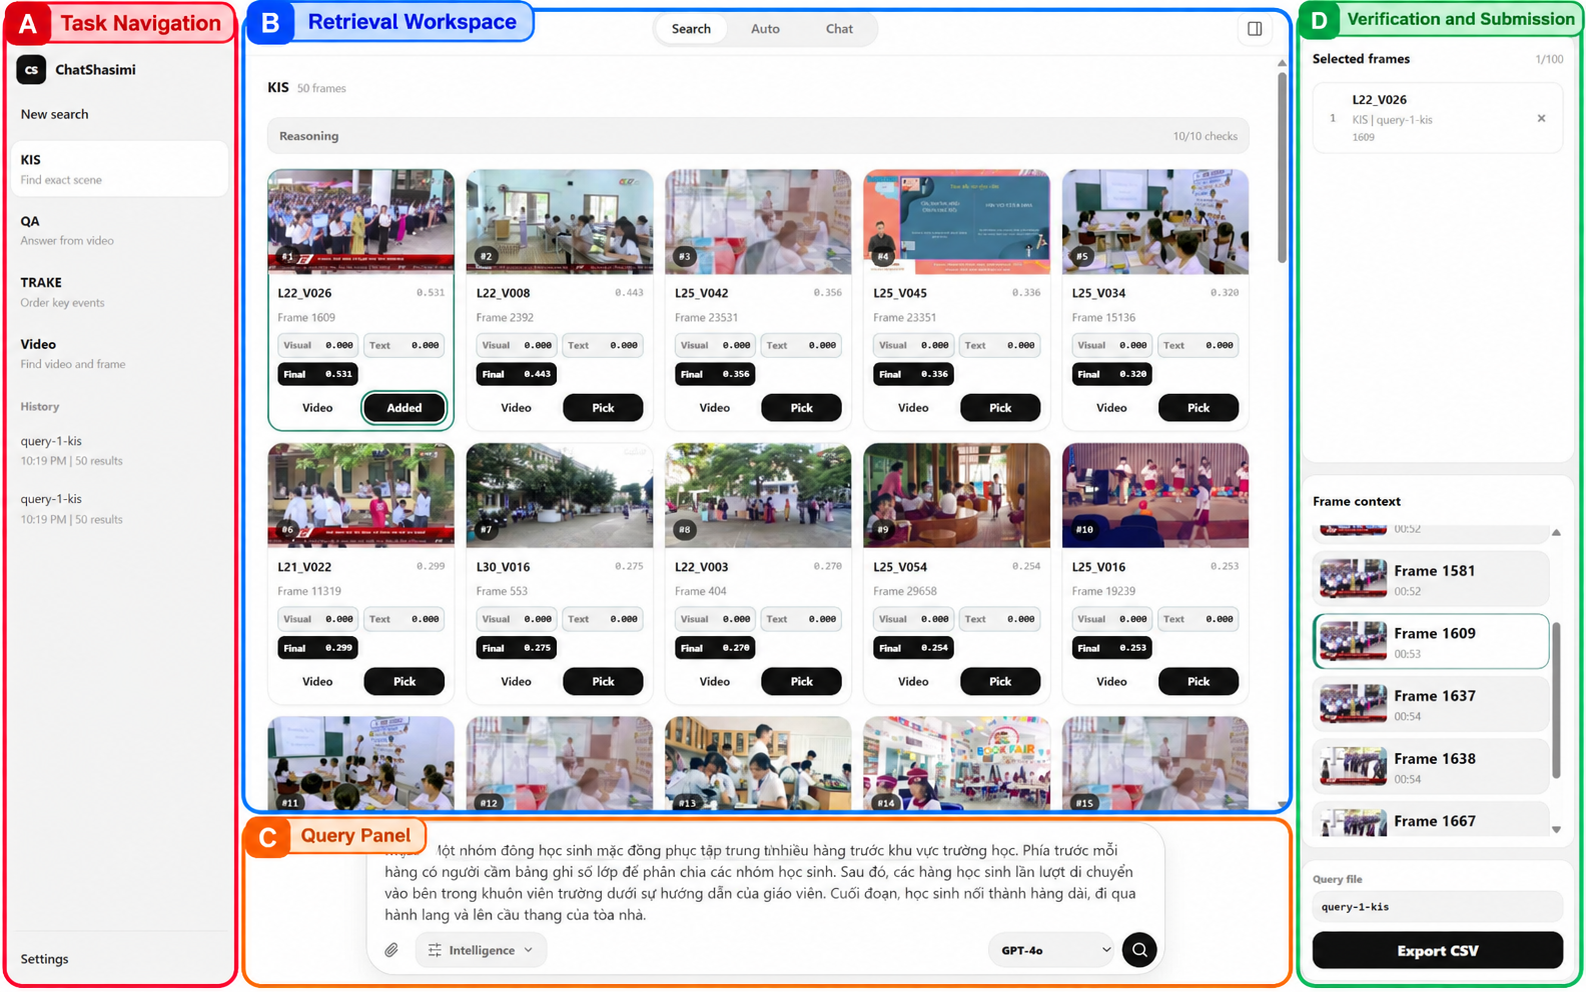
\includegraphics[width=\textwidth]{figures/aic_2026_ui_v2.jpg}
    \caption{Overview of the proposed video retrieval interface.
    (A) task navigation, (B) ranked retrieval results,
    (C) query input and search controls, and
    (D) frame verification, temporal context, and result export.}
    \label{fig:ui}
\end{figure*}
\fi


% \subsection{Data Preprocessing}
% \subsection{Semantic Vector Retrieval}
% \subsection{Metadata Retrieval}
% \subsection{Adaptive Temporal Search}
% \subsection{Multiperspective LLM-based Search}
% \subsection{User Interface}
\section{Experiments}

\paragraph{\textbf{Research question.}}
The experiments address three research questions. RQ1 investigates the
trade-offs between retrieval effectiveness and latency of video-first
retrieval with local temporal refinement versus direct temporal frame
retrieval. RQ2 examines how semantic embedding model choice and the number
of LLM-generated query perspectives affect retrieval effectiveness and
latency. RQ3 assesses the sensitivity of retrieval performance to individual
components of the LLM retrieval-planner prompt.
% \begin{itemize}
%     \item RQ1: What are the effectiveness and latency trade-offs of retrieving videos first and refining frame details afterwards, compared with direct temporal frame retrieval?

%     \item RQ2: How do the choice of semantic embedding model and the number of LLM-generated query perspectives affect retrieval effectiveness and latency?

%     \item RQ3: How sensitive is retrieval performance to individual components of the LLM retrieval-planner prompt?
% \end{itemize}


% \subsection{Ablation Study}
% \label{sec:ablation}
\subsection{Temporal search algorithms (RQ1)}
\paragraph{Experimental setup} We construct an evaluation set of 78 AIC 2026 ground-truth queries,
comprising 58 temporal KIS queries and 20 QA queries.\footnote{Recall@$k$ measures whether the result is retrieved within the first $k$ candidates.}. We evaluated with Recall@$k$ for $k\in\{1,5,10,20,50,100\}$ and median latency.We compare three temporal retrieval methods: ATS, Vortex, and DEV. DEV performs global retrieval and video selection before local frame refinement. All runs use the recorded fixed configuration: GPT-4o planning, SigLIP2 visual search, temporal mode enabled, top-$100$ retrieval.


\begin{table}[t]
    \centering
    \caption{Recall@k and latency comparison for temporal search strategies.}
    \label{tab:temporal-recall}
    \small
    \setlength{\tabcolsep}{4pt}
    \begin{tabular}{lrrrrrrr}
        \toprule
        Method & R@1 & R@5 & R@10 & R@20 & R@50 & R@100 & Latency (ms) \\
        \midrule
        ATS
        & \textbf{41.03}
        & \textbf{64.10}
        & 67.95
        & 73.08
        & 78.21
        & 80.77
        & 13320.0 \\

        Vortex
        & 37.18
        & 61.54
        & 69.23
        & 75.64
        & 82.05
        & 88.46
        & \textbf{10832.5} \\

        DEV
        & 34.62
        & 60.26
        & \textbf{76.92}
        & \textbf{82.05}
        & \textbf{85.90}
        & \textbf{93.59}
        & 37410.0 \\
        \bottomrule
    \end{tabular}
\end{table}


\paragraph{Result}
Table~\ref{tab:temporal-recall} shows that ATS performs best at early
ranks, achieving the highest R@1 and R@5. In contrast, DEV obtains the
best recall from R@10 onward, reaching $93.59\%$ at R@100, compared
with $88.46\%$ for Vortex and $80.77\%$ for ATS. This indicates that
DEV preserves more relevant candidates at larger retrieval depths.

However, this improvement comes with higher computational cost.
DEV has a median latency of $37{,}410$~ms, compared with
$13{,}320$~ms for ATS and $10{,}832.5$~ms for Vortex, showing a
trade-off between retrieval recall and runtime efficiency.



\subsection{Semantic embedding models (RQ2)}

\paragraph{Experimental setup} We evaluate the effect of the visual encoder and LLM-generated
multi-view query expansion on semantic retrieval. The ablation
is conducted on 58 queries using the two visual encoders supported by
our system, OpenCLIP and SigLIP2. For each encoder, we compare the
original full query with perspective-based retrieval using
$n \in \{3,5,7\}$ semantic views.\footnote{Retrieval effectiveness is measured
using mean reciprocal rank (MRR), Recall@10 (R@10), and Recall@100
(R@100).} We additionally report mean retrieval latency to quantify the
computational cost of increasing the number of perspectives.

\begin{table}[t]
    \centering
    \caption{Visual encoder choice and multi-perspective query expansion over 58 queries.}
    \label{tab:query_ablation}
    \small
    \setlength{\tabcolsep}{3.8pt}
    \renewcommand{\arraystretch}{1.08}
    \begin{tabular}{llccccc}
        \toprule
        Encoder & Mode & $n$ &
        MRR $\uparrow$ &
        R@10 $\uparrow$ &
        R@100 $\uparrow$ &
        Lat. (ms) $\downarrow$ \\
        \midrule

        OpenCLIP
        & Full & 1
        & 0.0382
        & 0.0862
        & 0.1034
        & \textbf{150.1} \\

        & View. & 3
        & 0.0067
        & 0.0172
        & 0.0690
        & \textbf{207.7} \\

        & View. & 5
        & 0.0062
        & 0.0172
        & 0.0517
        & \textbf{229.7} \\

        & View. & 7
        & 0.0062
        & 0.0172
        & 0.0517
        & \textbf{247.6} \\

        \midrule

        SigLIP2
        & Full & 1
        & \textbf{0.0617}
        & \textbf{0.1034}
        & \textbf{0.1379}
        & 158.3 \\

        & View. & 3
        & \textbf{0.0371}
        & \textbf{0.1034}
        & \textbf{0.1379}
        & 210.7 \\

        & View. & 5
        & \textbf{0.0371}
        & \textbf{0.1034}
        & \textbf{0.1379}
        & 230.8 \\

        & View. & 7
        & \textbf{0.0369}
        & \textbf{0.0862}
        & \textbf{0.1379}
        & 249.7 \\

        \bottomrule
    \end{tabular}
\end{table}

\paragraph{Result} As shown in Table~\ref{tab:query_ablation}, full-query retrieval
outperforms multi-perspective expansion for OpenCLIP, while also
achieving lower latency. SigLIP2 is more robust: three or five
perspectives preserve R@10 and R@100, although MRR decreases.
Overall, SigLIP2 with the full query achieves the strongest retrieval
effectiveness, whereas OpenCLIP with the full query provides the lowest
latency. Increasing the number of perspectives beyond three yields no
additional recall gains and consistently increases latency.

% \subsection{Prompt versions for LLM Retrieval Planner (RQ3)}

% \label{subsec:llm-prompt-component-ablation}

% We hold the retrieval stack fixed and ablate the planner prompt. The complete repository prompt is the \emph{Full Prompt}; each variant removes one configured component $C_i$. The components are C1 meaning preservation, C2 clause classification, C3 global weights, C4 text routing, C5 modality preference, C6 English semantic views, C7 Vietnamese lexical views, C8 OCR preservation, C9 observable terms, C10 rewrite length, C11 root rewrite, C12 temporal-KIS planning, C13 task-specific event structure (including ordered-query and TRAKE constraints), and C14 event weighting. 
% % TO-DO: They constrain the structured retrieval plan; chain-of-thought is not evaluated.

% % TO-DO: The fixed AIC 2025--2026 benchmark contains 98 queries (75 KIS and 23 retrieval-only QA) and no TRAKE samples. 
% We use \texttt{gpt-4o-mini}, temperature 0.05, and a 2,048-token output limit. Three repetitions over 15 conditions yield $15\times3\times98=4{,}410$ successful canonical records. All other retrieval settings are fixed (SigLIP2, strict hybrid top-$100$, metadata enabled, temporal mode for KIS, and reranking and query expansion disabled).
% % TO-DO: ; QA answer generation is disabled.

% For each query, video-level Recall@$k$ indicates whether the first $k$ results contain the ground-truth video. The primary outcome is the unweighted mean of Recall@1, @5, @20, @50, and @100 (MeanR). Exact-frame recall, using the single annotated frame, is secondary and is averaged over the same cutoffs. We define $\Delta=\text{ablation}-\text{Full}$. Repetitions are first averaged within query and condition, after which Full and each ablation are paired by query.

% We use 10,000 paired bootstrap samples for the 95\% CI and 20,000 paired random sign flips for the two-sided $p$-value.

% The Full Prompt obtains Recall@1, @5, @20, @50, and @100 of 35.71\%, 51.70\%, 70.41\%, 73.81\%, and 77.21\%, respectively, giving a MeanR of 61.77\% and mean exact-frame recall of 5.71\%. Table~\ref{tab:llm-prompt-ablation} reports all 14 removals.

% \begin{table}[t]

% \centering

% \caption{Leave-one-component-out planner-prompt ablation. MeanR is in percent; $\Delta$ and 95\% CIs are percentage points relative to Full.}

% \label{tab:llm-prompt-ablation}

% \scriptsize

% \setlength{\tabcolsep}{1.8pt}

% \renewcommand{\arraystretch}{1.02}

% \begin{tabular}{lrrrr@{\hspace{5pt}}lrrrr}

% \toprule

% \textbf{ID} & \textbf{MeanR} & \textbf{$\Delta$} & \textbf{95\% CI} & \textbf{$p$} &
% \textbf{ID} & \textbf{MeanR} & \textbf{$\Delta$} & \textbf{95\% CI} & \textbf{$p$} \\

% \midrule

% C1 & 62.31 & +0.54 & $[-2.38,3.54]$ & .755 & C8 & 63.27 & +1.50 & $[-2.04,5.10]$ & .449 \\

% C2 & 63.95 & +2.18 & $[-1.70,6.12]$ & .292 & C9 & 60.75 & -1.02 & $[-5.10,2.79]$ & .646 \\

% C3 & 63.74 & +1.97 & $[-1.36,5.37]$ & .276 & C10 & 63.74 & +1.97 & $[-1.77,6.05]$ & .344 \\

% C4 & 63.33 & +1.56 & $[-2.38,5.65]$ & .473 & C11 & 64.42 & +2.65 & $[-0.75,6.26]$ & .160 \\

% C5 & 62.72 & +0.95 & $[-2.38,4.35]$ & .611 & C12 & 63.88 & +2.11 & $[-2.11,6.19]$ & .339 \\

% C6 & 63.54 & +1.77 & $[-3.27,7.01]$ & .527 & C13 & 63.40 & +1.63 & $[-1.97,5.31]$ & .415 \\

% C7 & 60.34 & -1.43 & $[-5.03,2.04]$ & .466 & C14 & 62.99 & +1.22 & $[-3.27,5.78]$ & .626 \\

% \bottomrule

% \end{tabular}

% \end{table}

% All CIs include zero and all sign-flip tests have $p>.05$; hence, no component effect is statistically conclusive at the 5\% level. Twelve removals have positive MeanR point estimates, whereas C7 and C9 are negative. C7 gives the largest directional decrease ($-1.43$ points; $-2.58$ within KIS), while C9 reduces MeanR by 1.02 points and mean exact-frame recall by 1.84 points. These subgroup patterns are descriptive, especially for the 23-query QA subset, and measure conditional sensitivity within the complete prompt rather than isolated causal importance.

% MeanR can hide ranking-depth trade-offs: removing C3 increases MeanR by 1.97 points and Recall@5 by 6.46 points but decreases Recall@1 by 3.74 points; removing C12 increases MeanR by 2.11 points and Recall@100 by 6.12 points while decreasing Recall@1 by 3.40 points and mean exact-frame recall by 3.13 points.

% Thus, a positive delta does not imply improvement at every rank or that a component is unnecessary, particularly because prompt components may interact.

% The 14 related tests are unadjusted for multiplicity, but all unadjusted $p$-values already exceed .05, so correction would not change the non-significance conclusion. No TRAKE-effectiveness claim can be made from this benchmark; the small QA subset and single-reference exact-frame metric further limit generalization.

\subsection{Prompt components for LLM Retrieval Planner (RQ3)}
\label{subsec:llm-prompt-component-ablation}

We keep the retrieval stack fixed and perform leave-one-component-out ablation on the planner prompt. The \emph{Full Prompt} contains 14 components: C1 meaning preservation, C2 clause classification, C3 global weights, C4 text routing, C5 modality preference, C6 English semantic views, C7 Vietnamese lexical views, C8 OCR preservation, C9 observable terms, C10 rewrite length, C11 root rewrite, C12 temporal-KIS planning, C13 task-specific event structure, and C14 event weighting.

We use \texttt{gpt-4o-mini} with temperature 0.05 and a 2,048-token output limit. The experiment covers 98 queries and 15 prompt conditions, each repeated three times, yielding 4,410 runs. All other retrieval settings are fixed: SigLIP2, hybrid top-$100$ retrieval, metadata enabled, temporal mode for KIS, and reranking and query expansion disabled.

We evaluate video-level Recall@$k$ and define MeanR as the average of Recall@1, @5, @20, @50, and @100. Exact-frame recall over the same cutoffs is used as a secondary metric. We report $\Delta=\text{ablation}-\text{Full}$, with 95\% confidence intervals from 10,000 paired bootstrap samples and two-sided $p$-values from 20,000 paired sign-flip tests.

The Full Prompt achieves Recall@1, @5, @20, @50, and @100 of 35.71\%, 51.70\%, 70.41\%, 73.81\%, and 77.21\%, respectively, corresponding to a MeanR of 61.77\% and mean exact-frame recall of 5.71\%. Table~\ref{tab:llm-prompt-ablation} summarizes all ablations.

\begin{table}[t]
\centering
\caption{Leave-one-component-out planner-prompt ablation. MeanR is in percent; $\Delta$ and 95\% CIs are percentage points relative to Full.}
\label{tab:llm-prompt-ablation}
\scriptsize
\setlength{\tabcolsep}{4.8pt}
\renewcommand{\arraystretch}{1.02}
\begin{tabular}{lrrrr@{\hspace{5pt}}lrrrr}
\toprule
\textbf{ID} & \textbf{MeanR} & \textbf{$\Delta$} & \textbf{95\% CI} & \textbf{$p$} &
\textbf{ID} & \textbf{MeanR} & \textbf{$\Delta$} & \textbf{95\% CI} & \textbf{$p$} \\
\midrule
C1 & 62.31 & +0.54 & $[-2.38,3.54]$ & .755 & C8 & 63.27 & +1.50 & $[-2.04,5.10]$ & .449 \\
C2 & 63.95 & +2.18 & $[-1.70,6.12]$ & .292 & C9 & 60.75 & -1.02 & $[-5.10,2.79]$ & .646 \\
C3 & 63.74 & +1.97 & $[-1.36,5.37]$ & .276 & C10 & 63.74 & +1.97 & $[-1.77,6.05]$ & .344 \\
C4 & 63.33 & +1.56 & $[-2.38,5.65]$ & .473 & C11 & 64.42 & +2.65 & $[-0.75,6.26]$ & .160 \\
C5 & 62.72 & +0.95 & $[-2.38,4.35]$ & .611 & C12 & 63.88 & +2.11 & $[-2.11,6.19]$ & .339 \\
C6 & 63.54 & +1.77 & $[-3.27,7.01]$ & .527 & C13 & 63.40 & +1.63 & $[-1.97,5.31]$ & .415 \\
C7 & 60.34 & -1.43 & $[-5.03,2.04]$ & .466 & C14 & 62.99 & +1.22 & $[-3.27,5.78]$ & .626 \\
\bottomrule
\end{tabular}
\end{table}

All confidence intervals include zero and all $p$-values exceed .05, so no individual component shows a statistically significant effect at the 5\% level. C7 and C9 are the only removals that reduce MeanR, by 1.43 and 1.02 points, respectively; C9 also reduces mean exact-frame recall by 1.84 points.

The results also reveal ranking-depth trade-offs. Removing C3 improves MeanR and Recall@5 but reduces Recall@1, while removing C12 improves MeanR and Recall@100 but decreases both Recall@1 and exact-frame recall. Thus, a positive MeanR change does not imply consistent improvement across ranking depths or that a component is unnecessary, particularly because prompt components may interact.

Because all unadjusted $p$-values exceed .05, multiplicity correction would not change the significance conclusion. Moreover, the benchmark contains no TRAKE samples, while the QA subset and single-reference exact-frame evaluation are limited; therefore, these results should be interpreted as prompt-sensitivity analysis rather than isolated causal effects.

\subsection{Analysis}
Table~\ref{tab:official-results} summarizes the official preliminary-round
results of our system in the AIC 2026 Multimodal Retrieval Challenge.
The system achieved scores of 21.27, 27.20, and 27.75 across the three
evaluation rounds, corresponding to 88.63\%, 93.79\%, and 84.09\% of
the maximum scores, respectively. Overall, the system obtained
76.22 out of 86 points, equivalent to 88.63\% of the total available
score. The results demonstrate the effectiveness of the proposed
multimodal and temporal retrieval pipeline across multiple evaluation
rounds. The lower relative performance in Round~3 indicates that
further improvements are still possible for more complex retrieval
scenarios.

\begin{table}[t]
\centering
\caption{Official preliminary-round results on the AIC 2026 benchmark.}
\label{tab:official-results}
\small
\begin{tabular}{lccc}
\hline
\textbf{Round} & \textbf{Official Score} & \textbf{Maximum Score} & \textbf{Score (\%)} \\
\hline
Round 1 & 21.27 & 24 & 88.63\% \\
Round 2 & 27.20 & 29 & 93.79\% \\
Round 3 & 27.75 & 33 & 84.09\% \\
\hline
\textbf{Overall} & \textbf{76.22} & \textbf{86} & \textbf{88.63\%} \\
\hline
\end{tabular}
\end{table}



\section{Conclusion}
\label{sec:conclusion}

In this work, we introduced a multimodal video retrieval system for the AI Challenge 2026 that combines LLM-assisted retrieval planning, multimodal evidence fusion, and explicit temporal reasoning. By integrating complementary visual representations with OCR, ASR, caption, and object-level metadata, the system supports both semantic and lexical retrieval across diverse query types. We further proposed Diagnostic-Event-Video-First (DEV), a coarse-to-fine temporal retrieval strategy that first identifies promising videos and then performs event-level refinement under chronological and temporal-gap constraints.

Experimental results demonstrate the effectiveness of the proposed design. DEV achieves $93.59\%$ R@100, showing strong recall at larger retrieval depths, while the complete system obtains $88.63\%$ of the maximum score in the AIC 2026 preliminary evaluation. These results indicate that combining query-aware multimodal retrieval with explicit temporal sequence construction is effective for complex video retrieval scenarios.

Despite these results, challenges remain in early-rank retrieval, computational efficiency, and complex multi-event scenarios. The current one-shot LLM planner may also produce redundant or suboptimal query reformulations. In future work, we plan to investigate an agentic retrieval framework that can iteratively observe intermediate evidence, select appropriate visual, textual, and temporal retrieval tools, and adapt its strategy during retrieval. We also aim to improve early-rank precision and reduce retrieval latency while preserving temporal consistency and multimodal robustness.



% \subsection{A Subsection Sample}
% Please note that the first paragraph of a section or subsection is
% not indented. The first paragraph that follows a table, figure,
% equation etc. does not need an indent, either.

% Subsequent paragraphs, however, are indented.

% \subsubsection{Sample Heading (Third Level)} Only two levels of
% headings should be numbered. Lower level headings remain unnumbered;
% they are formatted as run-in headings.

% \paragraph{Sample Heading (Fourth Level)}
% The contribution should contain no more than four levels of
% headings. Table~\ref{tab1} gives a summary of all heading levels.

% \begin{table}
% \caption{Table captions should be placed above the
% tables.}\label{tab1}
% \begin{tabular}{|l|l|l|}
% \hline
% Heading level &  Example & Font size and style\\
% \hline
% Title (centered) &  {\Large\bfseries Lecture Notes} & 14 point, bold\\
% 1st-level heading &  {\large\bfseries 1 Introduction} & 12 point, bold\\
% 2nd-level heading & {\bfseries 2.1 Printing Area} & 10 point, bold\\
% 3rd-level heading & {\bfseries Run-in Heading in Bold.} Text follows & 10 point, bold\\
% 4th-level heading & {\itshape Lowest Level Heading.} Text follows & 10 point, italic\\
% \hline
% \end{tabular}
% \end{table}


% \noindent Displayed equations are centered and set on a separate
% line.
% \begin{equation}
% x + y = z
% \end{equation}
% Please try to avoid rasterized images for line-art diagrams and
% schemas. Whenever possible, use vector graphics instead (see
% Fig.~\ref{fig1}).

% \begin{figure}
% 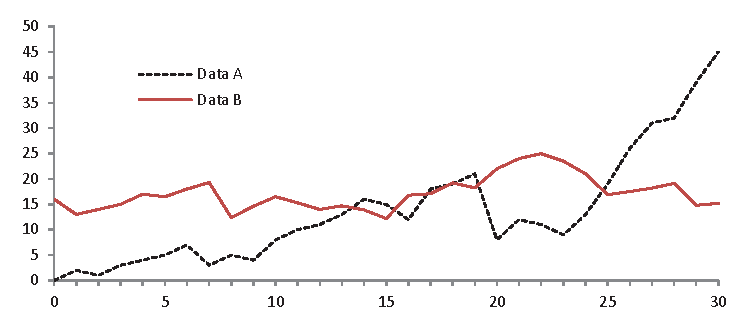
\includegraphics[width=\textwidth]{fig1.eps}
% \caption{A figure caption is always placed below the illustration.
% Please note that short captions are centered, while long ones are
% justified by the macro package automatically.} \label{fig1}
% \end{figure}

% \begin{theorem}
% This is a sample theorem. The run-in heading is set in bold, while
% the following text appears in italics. Definitions, lemmas,
% propositions, and corollaries are styled the same way.
% \end{theorem}
% %
% % the environments 'definition', 'lemma', 'proposition', 'corollary',
% % 'remark', and 'example' are defined in the LLNCS documentclass as well.
% %
% \begin{proof}
% Proofs, examples, and remarks have the initial word in italics,
% while the following text appears in normal font.
% \end{proof}
% For citations of references, we prefer the use of square brackets
% and consecutive numbers. Citations using labels or the author/year
% convention are also acceptable. The following bibliography provides
% a sample reference list with entries for journal
% articles~\cite{ref_article1}, an LNCS chapter~\cite{ref_lncs1}, a
% book~\cite{ref_book1}, proceedings without editors~\cite{ref_proc1},
% and a homepage~\cite{ref_url1}. Multiple citations are grouped
% \cite{ref_article1,ref_lncs1,ref_book1},
% \cite{ref_article1,ref_book1,ref_proc1,ref_url1}.

% \begin{credits}
% \subsubsection{\ackname} A bold run-in heading in small font size at the end of the paper is
% used for general acknowledgments, for example: This study was funded
% by X (grant number Y).

\section*{Acknowledgement}
This research is supported by research funding from Faculty of Information Technology, University of Science, Vietnam National University - Ho Chi Minh City.
% \subsubsection{\discintname}
% It is now necessary to declare any competing interests or to specifically
% state that the authors have no competing interests. Please place the
% statement with a bold run-in heading in small font size beneath the
% (optional) acknowledgments\footnote{If EquinOCS, our proceedings submission
% system, is used, then the disclaimer can be provided directly in the system.},
% for example: The authors have no competing interests to declare that are
% relevant to the content of this article. Or: Author A has received research
% grants from Company W. Author B has received a speaker honorarium from
% Company X and owns stock in Company Y. Author C is a member of committee Z.
% \end{credits}
%
% ---- Bibliography ----
%
% BibTeX users should specify bibliography style 'splncs04'.
% References will then be sorted and formatted in the correct style.
%
\bibliographystyle{splncs04}
\bibliography{references}

\end{document}
